\documentclass{article}
\usepackage{pdfpages}
\usepackage[german]{babel}
\usepackage{hyperref}
\usepackage[utf8]{inputenc}
\usepackage{xcolor}
\usepackage{fancyhdr}
%\usepackage{multicol}

\usepackage{caption}
\usepackage{subcaption}

\usepackage{amsmath}
\usepackage{amssymb}
\usepackage{amsfonts}
\usepackage{mathtools}
\usepackage{svg}

\usepackage[]{algorithm2e}

\usepackage{biblatex}
\addbibresource{sources.bib}

\newcommand{\pro}{\ensuremath{+}}
\newcommand{\contra}{\ensuremath{-}}

\pagestyle{fancy} %eigener Seitenstil
\fancyhf{} %alle Kopf- und Fußzeilenfelder bereinigen
\fancyhead[L]{\today} %Kopfzeile links
\fancyhead[C]{Zufällige Partitionen} %zentrierte Kopfzeile
\fancyhead[R]{Stefan Volz} %Kopfzeile rechts
\renewcommand{\headrulewidth}{0.4pt} %obere Trennlinie
\fancyfoot[C]{\thepage} %Seitennummer
\renewcommand{\footrulewidth}{0.4pt} %untere Trennlinie

\setcounter{tocdepth}{2}
\setlength{\parindent}{0pt}

\title{Generation zufälliger Partitionen}
\author{Stefan Volz}

\newtheorem{definition}{Definition}
\newtheorem{notation}{Notation}
\newtheorem{theorem}{Satz}
\newtheorem{lemma}{Lemma}
\newtheorem{corollary}{Korollar}
\newtheorem{proof}{Beweis}

\newcommand{\underbraced}[2]{\ensuremath{\underset{#2}{\underbrace{#1}}}}

\begin{document}

\begin{titlepage}
    \maketitle

    \begin{abstract}
        Wir bezeichnen ein $k$-Tupel $(c_1,...,c_k) \in \mathbb{N}_0^k$ mit Elementen $c_i \leq r \in \mathbb{N}$ als geordnete $r$-beschränkte $k$-Partition von $n \in \mathbb{N}$, wenn $\sum_{j=1}^k c_j = n$. Bezeichne mit $\mathcal{P}_k^r(n)$ die Menge dieser Partitionen. Gesucht wird ein effizienter Algorithmus um gleichverteilt ein zufälliges Element aus $\mathcal{P}_k^r(n)$ zu generieren.
    \end{abstract}

    \tableofcontents
\end{titlepage}
\setcounter{page}{2}

\section{Unbeschränkte Partitionen}
Betrachten wir zunächst die Menge der unbeschränkten Partitionen $\mathcal{P}_k^n(n) =: \mathcal{P}_k(n)$.
\begin{notation}
    Wir bezeichnen die Anzahl an unbeschränkten Partitionen mit $\psi_k(n)$ und nennen $k$ die Dimension dieser Partitionen.
\end{notation}

\subsection{Motivation}

Betrachten wir $\mathcal{P}_k(n)$ als die Menge der Lösungen $(x_1, ... , x_k)$ der Gleichung $x_1 + ... + x_k = n$, so liegen diese geometrisch betrachtet alle auf der durch selbige Gleichung definierten Hyperebene.

\begin{figure}[ht]
    \centering
    \begin{subfigure}{.5\textwidth}
        \centering
        \includesvg[width=\textwidth, keepaspectratio]{./img/2d1.svg}
        \caption{Beispiel für $k=2, n=5$}
        \label{fig:2d1}
    \end{subfigure}%
    \begin{subfigure}{.5\textwidth}
        \centering
        \includesvg[width=\textwidth, keepaspectratio]{./img/3d1.svg}
        \caption{Beispiel für $k=3, n=5$}
        \label{fig:3d1}
    \end{subfigure}
    \caption{Geometrische Veranschaulichung der unbeschränkten Partitionen}
    \label{fig:unboundedpartitions}
\end{figure}

Dieses Bild legt nahe, dass sich die Anzahl an 3-dimensionalen Partitionen aus der Anzahl an 2-dimensionalen Partitionen zusammensetzt - also eine rekursive Beziehung zwischen $\psi_3$ und $\psi_2$ besteht. Setzen wir z.B. $x_3$ auf einen festen Wert, so folgt
\begin{align*}
    x_1 + x_2 = n - x_3,
\end{align*}
also ist $(x_1, x_2)$ eine $2$-Partition von $n-x_3$ wenn $(x_1, x_2, x_3)$ eine $3$-Partition von $n$ ist. Da $x_3$ alle Werte in $\{0,...,n\}$ annehmen kann ergibt sich somit
\begin{align}
    \psi_3(n) = \sum_{x_3=0}^n \psi_2(n-x_3) \underset{r:=n-x_3}{=} = \sum_{r=0}^n \psi_2(r) \label{eq:psi3}.
\end{align}
Für den $\psi_2$ finden wir mittels kombinatorischer Argumente (die Menge $\{0,...,n\}$ hat $n+1$ Elemente, wir wählen hieraus eines für $x_2$ aus und definieren somit eindeutig eine Partition. Es gibt $\begin{pmatrix}
        n+1 \\ 1
    \end{pmatrix} = n+1$ Möglichkeiten diese Auswahl zu treffen.) $\psi_2(n) = n+1$. Mit Rückblick auf Gleichung \ref{eq:psi3} schreiben wir dies als
\begin{align}
    \psi_2(n) = n+1 = \sum_{r=0}^n 1 = \sum_{r=0}^n \psi_1(n),
\end{align}
wobei wir $\psi_1(n) = 1$ als trivial wahr erkennen.
Dies legt die generelle Formel
\begin{align}
    \psi_{k+1}(n) = \sum_{r=0}^k \psi_k(n), ~~~~ \text{mit } k \in \mathbb{N}, n \in \mathbb{N}_0 \label{eq:psi_k_recursive}
\end{align}
nahe, von deren Gültigkeit wir uns auch in höheren Dimensionen leicht überzeugen (Setzen wir einen Freiheitsgrad auf $r \in \{0,...,n\}$ fest so müssen die restlichen eine beliebige $k$-Partition von $n-r$ bilden.).

\subsection{Geschlossene Form von $\psi_k(n)$}

Berechnen wir nach obiger Formel $\psi_k(n)$ für einige $k$ erhalten wir:
\begin{align*}
    \psi_1(n) = \hphantom{\frac{1}{2}(}  & \hphantom{n+} 1     \\
    \psi_2(n) = \hphantom{\frac{1}{2}} ( & n+1)                \\
    \psi_3(n) = \frac{1}{2} (            & n+1)(n+2)(n+3)      \\
    \psi_4(n) = \frac{1}{6} (            & n+1)(n+2)(n+3)(n+4)
\end{align*}
was die Vermutung
\begin{align}
    \psi_k(n) = \frac{1}{(k-1)!} \prod_{r=1}^{k-1}(n+r) \label{eq:psikn}
\end{align}
nahelegt. Da es nicht völlig trivial ist die Gültigkeit dieser Formel anhand Gleichung \ref{eq:psi_k_recursive} zu beweisen, wollen wir sie mittels generierenden Funktionen herleiten.
Sei daher
\begin{align*}
    G_n(x) := \sum_{k=1}^\infty \psi_k(n) x^k
\end{align*}
die Familie der gewöhnlichen generierenden Funktionen den Folgen $(\psi_k(n))_{k \in \mathbb{N}}$ für $n \in \mathbb{N}_0$. Multiplizieren wir Gleichung \ref{eq:psi_k_recursive} beidseitig mit $x^k$ und summieren über ihren Gültigkeitsbereich in $k$ erhalten wir
\begin{align*}
    \frac{1}{x}\sum_{k=1}^\infty \psi_k(n) x^k - \psi_1(n) & = \sum_{k=1}^\infty \sum_{r=0}^n x^k \psi_k(n) = \sum_{r=0}^n \sum_{k=1}^\infty x^k \psi_k(n) \\
    \iff G_n(x)                                            & = x (\sum_{r=0}^n G_r(x) - \psi_1(n)).
\end{align*}
Durch abspalten des letzten Terms der rechtsseitigen Summe und anschließendes Auflösen nach $G_n(x)$ erhalten wir
\begin{align}
    G_n(x) = \frac{x}{1-x} (\sum_{r=0}^{n-1} G_r(x) + \psi_1(n)).
\end{align}
Wir berechnen die $G_n$ mittels dieser Formel und
\begin{align*}
    G_0(x) \underset{\psi_1(n)=1}{=} \sum_{k=1}^\infty x^k = \frac{1}{1-x} - 1 = \frac{x}{1-x}
\end{align*}
für einige $n$:
\begin{align*}
    G_1(x) = \frac{x}{(1-x)^2} \\
    G_2(x) = \frac{x}{(1-x)^3} \\
    G_3(x) = \frac{x}{(1-x)^4}.
\end{align*}
Es liegt nahe, dass \begin{align}
    G_n(x) = \frac{x}{(1-x)^{n+1}}. \label{eq:Gn}
\end{align}

Sei $g(x) := \frac{1}{1-x}$. Nach der Cauchy-Produktformel gilt
\begin{align*}
    g(x)^2 = \frac{1}{1-x} \cdot \frac{1}{1-x} = \sum_{k=0}^\infty \sum_{r=0}^k x^r x^{k-r} = \sum_{k=0}^\infty (k+1)x^k = Dg(x).
\end{align*}
Somit gilt $D(g^n(x)) = ng^{n-1}(x) Dg(x) = ng^{n+1}(x)$ woraus wir
\begin{align*}
    g^{n+1}(x)      = \frac{1}{n} D g^n(x) & = \frac{1}{n(n-1)} D^2 g^{n-1}(x) = ... = \frac{1}{n!} D^n g(x) \\
    \iff D^k g^n(x)                        & = (n)^{\bar{k}} g^{n+k}(x)
\end{align*}
erhalten, wobei $(n)^{\bar{k}}$ die steigende Faktorielle bezeichnet. Somit folgt für die Taylorentwicklung von $g^n$ um $0$
\begin{align*}
    g^n(x) = \sum_{k=0}^\infty \frac{D^k g^n(0)}{k!} x^k = \sum_{k=0}^\infty \frac{(n)^{\bar{k}} g^{n+k}(0)}{k!} x^k = \sum_{k=0}^\infty \frac{(n)^{\bar{k}}}{k!} x^k,
\end{align*}
womit wir für $G_n$ folgende Reihendarstellung erhalten
\begin{align*}
    G_n(x) = \sum_{k=0}^\infty \frac{(n+1)^{\bar{k}}}{k!} x^{k+1} = \sum_{k=1}^\infty \frac{(n+1)^{\overline{k-1}}}{(k-1)!} x^k.
\end{align*}
Durch Koeffizientenvergleich mit der ursprünglichen Definition der generierenden Funktion erhalten wir die in Gleichung \ref{eq:psikn} bereits vermutete Darstellung
\begin{align}
    \psi_k(n) = \frac{(n+1)^{\overline{k-1}}}{(k-1)!} = \frac{1}{(k-1)!} \prod_{r=0}^{k-2} (n+1+r) = \frac{1}{(k-1)!} \prod_{r=1}^{k-1} (n+r) \label{eq:psiknclosed}
\end{align}
welche für $k \geq 1, n \geq 0$ gültig ist.

\section{Beschränkte Partitionen}

Wenden wir uns nun den beschränkten Partitionen zu.
\begin{notation}
    Wir bezeichnen die Anzahl an $r$-beschränkten $k$-Partitionen mit $\varphi_k^r(n)$.
\end{notation}

\subsection{Motivation}
Wie auch zuvor können wir uns die beschränkten Partitionen geometrisch veranschaulichen.

\begin{figure}[ht]
    \centering
    \begin{subfigure}{.5\textwidth}
        \centering
        \includesvg[width=\textwidth, keepaspectratio]{./img/2d2.svg}
        \caption{Beispiel für $\varphi_2^4(5)=4$}
        \label{fig:2d2}
    \end{subfigure}%
    \begin{subfigure}{.5\textwidth}
        \centering
        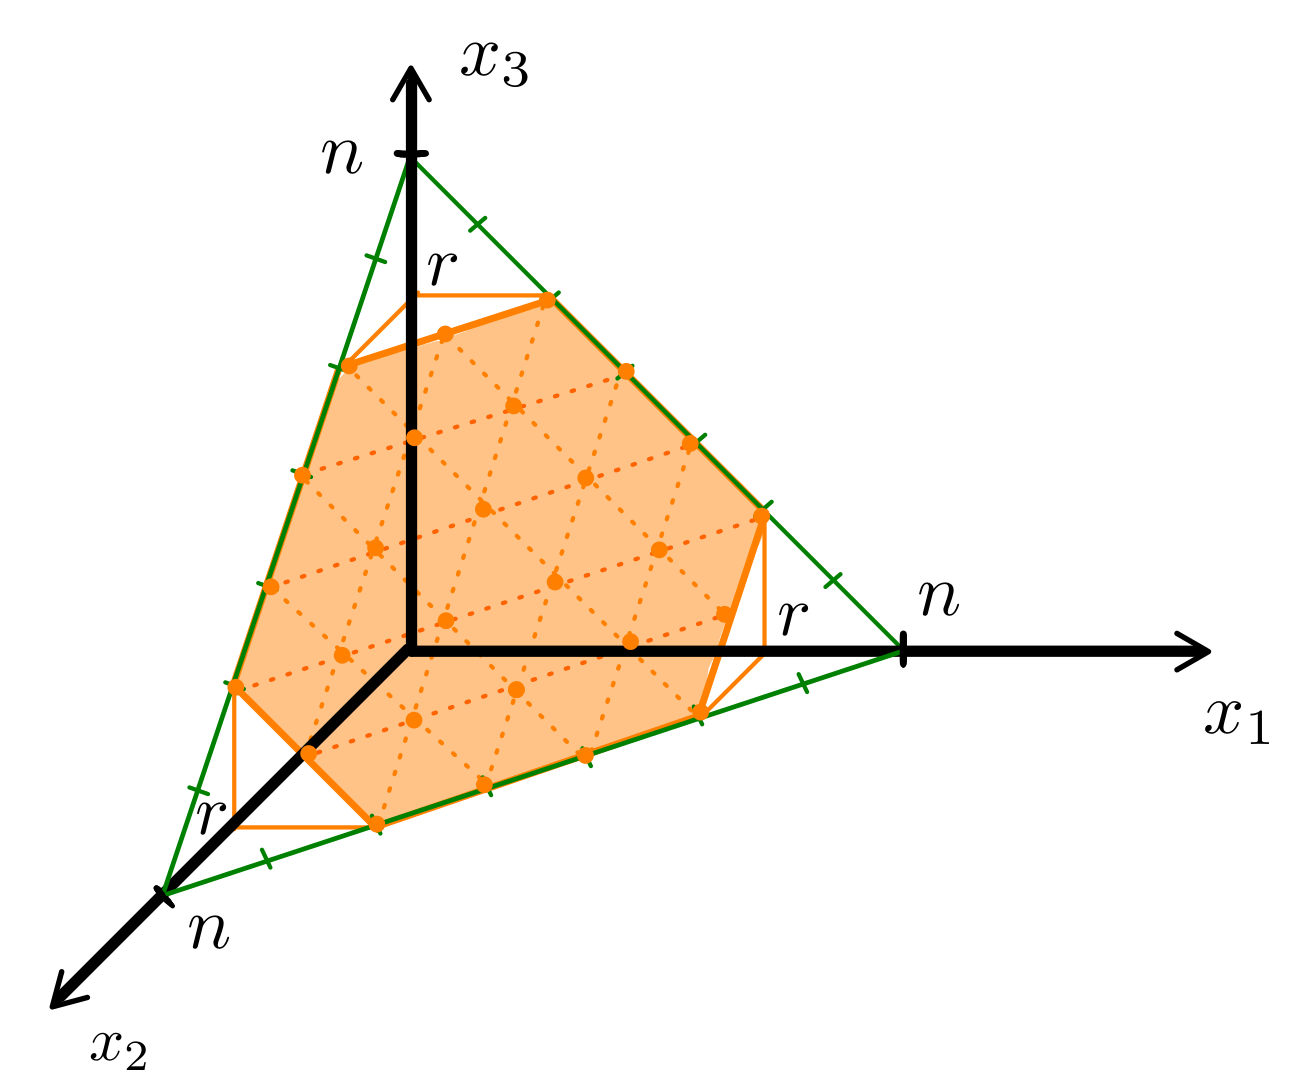
\includegraphics[width=\textwidth, keepaspectratio]{./img/3d2.png}
        \caption{Beispiel für $k=3, n=7, r=5, \varphi_3^5(7)=27$}
        \label{fig:3d2}
    \end{subfigure}
    \caption{Geometrische Veranschaulichung der beschränkten Partitionen}
    \label{fig:boundedpartitions}
\end{figure}

Wir nehmen sozusagen alle unbeschränkten Partitionen, und schneiden dann die kleineren Teile weg, bei denen einzelne Komponenten die Schranke $r$ überschreiten würden.

\subsection{Wahrscheinlichkeitsverteilung der beschränkten Partitionen}

Diese Überlegungen können wir direkt in eine Gleichung übersetzen und erhalten somit
\begin{align*}
    \varphi_k^{r-1}(n) = \psi_k(n) - k\psi_k(n-r) \text{ mit } k \geq 1, n, n-r \geq 0.
\end{align*}
Hierbei erklärt sich der Index $(r-1)$ dadurch, dass wir die Elemente der ’’Schnittgrenze'' mitnehmen wollen.
Nehmen wir nun an, dass alle Partitionen gleichwahrscheinlich sind, so erhalten wir ein Laplaceexperiment. Es sei $\Omega := \mathcal{P}_k^r(n)$ die Ergebnismenge, sowie $\omega:=(X_1,...,X_k) \in \Omega$ eine Zufällige Partition. Da $X_j=m$ genau dann wenn die restlichen Komponenten eine $(k-1)$-Partition bilden (also $(X_1,...,X_{j-1}, X_{j+1},...X_k) \in \mathcal{P}_k^r(n-m)$), gibt es $\varphi_{k-1}^r$ Möglichkeiten für die Konfiguration von $\omega$. Es gilt demnach
\begin{align}
    p_k^r(n,m) := P(X_j=m) = \frac{\varphi_{k-1}^r(n-m)}{\varphi_k^r(n)} \label{eq:probability_phi}.
\end{align}

\subsection{Effiziente Bestimmung von $P(X_j=m)$}
Da in \ref{eq:psiknclosed} und somit auch in \ref{eq:probability_phi} viele Fakultäten vorkommen ist diese Darstellung nicht praktikabel umsetzbar. Wir beginnen damit die Situation erstmal noch etwas schlimmer zu machen indem wir die fallende Faktorielle mittels Fakultäten ausdrücken und erhalten
\begin{align*}
    \varphi_k^{r-1}(n) = \frac{(n+k-1)!}{n!(k-1)!} - k\frac{(n-r+k-2)!}{(n-(r+1))!(k-1)!} = \frac{\Gamma(n+k)}{n!\Gamma(k)} - k\frac{\Gamma(n-r+k-1)}{\Gamma(n-r)\Gamma(k)}
\end{align*}
Wenden wir auf die beiden Terme jeweils $\exp \circ \ln$ an, ergibt sich mit $\ln F := \ln \circ (\cdot!)$
\begin{align*}
    \varphi_k^{r-1}(n) & = \exp(\ln\psi_k(n)) - \exp(\ln(k\psi_k(n-r)))   \\
                       & = \exp(\ln\Gamma(n+k) - \ln F(n) - \ln\Gamma(k)) \\ &- \exp(\ln(k) + \ln\Gamma(n+k-(r+1)) - \ln\Gamma(n-r) - \ln\Gamma(k)).
\end{align*}
Die Funktion $\ln\Gamma$ lässt sich über eine asymptotische Entwicklung auf Basis der verallgemeinerten Stirlingformel
\begin{align*}
    \Gamma(x) = \sqrt{\frac{2\pi}{x}} \left(\frac{x}{e}\right)^x e^{\mu(x)} \text{ mit }x > 0, 0 < \mu(x) < \frac{1}{12x}
\end{align*}
gut und effizient approximieren, es gilt
\begin{align*}
    \ln\Gamma(x) = (x - \frac{1}{2}) \ln x - x + \frac{1}{2} \ln{2 \pi} + \frac{1}{12 x} + \frac{1}{360 x^3} + \mathcal{O}(x^{-4}).
\end{align*}
Da selbst eine Taylorentwicklung höherer Ordnung von $f : (x,y) \mapsto e^x - e^y$ (z.B. $T_2f(x,y,u,v) = e^u (1+x-u+\frac{(x-u)^2}{2}) - e^v (1+y-v+\frac{(y-v)^2}{2})$ mit $u,v = \frac{|a-b|}{2}$: $T_2f(x,y) = e^{\frac{|b-a|}{2}}(a-b)(1+\max\{a,b\})$), uns für ausreichend große Argumente in praktisch unbrauchbaren Größenordnungen lässt, ersetzen wir $\exp$ in diesen Ausdrücken durch die Taylorentwicklung erster Ordnung und erhalten somit
\begin{align*}
    \varphi_k^{r-1}(n) & \overset{\centerdot}{=} \ln\Gamma(n+k) - \ln F(n) - \ln\Gamma(k) \\ &- \ln k + \ln\Gamma(n+k-(r+1)) - \ln\Gamma(n-r) - \ln\Gamma(k)
\end{align*}
womit wir $P(X_j=m)$ effizient berechnen können. Hiermit können wir uns eine Zufallsverteilung generieren\footnote{Sofern es zu teuer ist die ganze Verteilung zu erzeugen könnte man ggf. durch lückenweises Sampling und anschließende Renormalisierung einzelne Zahlen erhalten. Man erzeuge also für $\nu \in \mathbb{N}$ zunächst $M := \{(\nu m, p_k^r(n, \nu m)) | 0 \leq \nu m \leq n\}$, N := $\{p | (\_, p) \in M\}$ und hieraus die Wahrscheinlichkeitsverteilung $\{(m, \frac{p}{\sum_{\rho \in N} \rho}) | (m,p) \in M\}$. Ggf. kann man nach Erzeugen einer Zahl iterativ mit einem kleineren $\nu$ eine Auswahl auf dem durch die erste Zufallszahl bestimmten Teilintervall durchführen.} und auf Basis dieser Zufallszahlen erzeugen.

\subsection{Implementierung}

Sofern man wirklich formal korrekt gleichverteilte vollständige Partitionen erzeugen will müsste man in jedem Schritt $j$ als Verteilung die Wahrscheinlichkeiten $P(X_j=m | X_{j-1}=x_{j-1},...,X_1=x_1), 0 \leq m \leq r$ nutzen.

Der tatsächlich implementierte Algorithmus geht wie folgt vor

\begin{algorithm}[H]
    \KwData{$n, m, k \in \mathbb{N}$}
    \KwResult{zufällige Partition $(x_1,...,x_m)$ von $n$ sodass $x_j <= k$}
    \SetKwFunction{sample}{sample}
    \SetKw{break}{break}
    \SetKw{true}{True}
    \SetKwRepeat{Do}{do}{while}
    Gewichte $\leftarrow$ Feld für $n+1$ natürliche Zahlen auf $0$ initialisiert \\
    \For{$i \leftarrow 0$ \KwTo $\min\{k,n\}$} {
        Gewicht($i$) $\leftarrow p_m^k($Rest, $i)$ \\
    }
    \Do{$\max$(Partition) $\leq k$ \CommentSty{\#Die generierte Partition ist gültig} }{
        Partition $=(x_1,...,x_m) \leftarrow$ Feld für $m$ natürliche Zahlen auf $0$ initialisiert \\
        Rest $\leftarrow n$ \\
        \For{$i \leftarrow 1$ \KwTo $m-1$}{
            \While(){\true}{
                r $\leftarrow$ \sample(Gewichte) \CommentSty{\#Generiere Zufallszahl nach gegebener Verteilung} \\
                \If(){
                    $r \leq $ Rest
                }{
                    Rest $\leftarrow \max\{0, $ Rest $ - r\}$ \\
                    $x_i \leftarrow r$ \\
                    \break
                }
            }
        }
        $x_m \leftarrow Rest$}
    \Return{Partition}
\end{algorithm}

\subsection{Bla}

Es sei \begin{align*}
    \rho_k^r(n,m) := \begin{cases}
        \varphi_{k-1}^r(n-m) & k > 1 \\
        \delta_{n,m}         & k = 1
    \end{cases} ~~~~, 0 \leq m \leq n
\end{align*}
die Anzahl an $r$-beschränkten $k$-Partitionen von $n$ bei denen ein Element den Wert $m$ besitzt (der Zähler von Gleichung \ref{eq:probability_phi}).

\section{Alternativer Ansatz}

Stellen wir zunächst $n \in \mathbb{N}$ als Summe $\underbraced{1 + 1 + ... + 1}{n\text{ mal}}$ dar. Diese Summe enthält $(n-1)$ \emph{plus}-Symbole. Wählen wir aus diesen $k-1$ aus und entfernen alle restlichen, so erhalten wir $k \in \mathbb{N}$ Blöcke aus Einsen welche wir zusammenaddieren können um eine $k$-Partition von $n$ zu erhalten - umgedreht können wir aus einer Partition auch immer so eine Folge konstruieren. Unser Auswahlargument bedeutet somit, dass
\begin{align*}
    \psi(n) = \begin{pmatrix}
        n-1 \\ k-1
    \end{pmatrix}.
\end{align*}
Wir rechnen leicht nach, dass dies mit Gleichung \ref{eq:psiknclosed} übereinstimmt. Aus \cite{wik} erhalten wir weiterhin folgendes Ergebnis

\begin{theorem}\label{theo:wik}
    Es sei $A \subseteq \mathbb{N}_0, k \in \mathbb{N}$ und $(a_n)_{n \in \mathbb{N}_0}$ die Folge der Anzahl $A$-elementigen $k$-Partitionen von $n$. Dann ist die generierende Funktion $F$ von $(a_n)$ gegeben durch
    \begin{align*}
        F(x) = \left(\sum_{\alpha \in A} x^\alpha\right)^k.
    \end{align*}
\end{theorem}

Hieraus folgt direkt

\begin{corollary}
    Die generierende Funktion $\Phi_k^r$ von $(\varphi_k^r(n))_{n \in \mathbb{N}_0}$ lautet
    \begin{align*}
        \Phi_k^r(x) = \left(\sum_{i=0}^r x^i \right)^k = \sum_{\sum_{i=1}^k \kappa_i = k} \begin{pmatrix} k \\ \kappa_1, ..., \kappa_k \end{pmatrix} \cdot \prod_{i=1}^k x^{\kappa_i}.
    \end{align*}
\end{corollary}

\begin{proof}
    Die Gleichung
    \begin{align*}
        \Phi_k^r(x) = \left(\sum_{i=0}^r x^i \right)^k
    \end{align*}
    folgt mit $A=\{0,...,r\}$ direkt aus Satz \ref{theo:wik}.
    Anwenden des Multinomialsatzes liefert uns
    \begin{align*}
        \left(\sum_{i=0}^r x^i\right)^k & = \sum_{\sum_{i=0}^r \kappa_i = k} \begin{pmatrix} k \\ \kappa_0, ..., \kappa_r \end{pmatrix} \cdot \prod_{i=0}^r (x^i)^{\kappa_i} \\
                                        & = \sum_{\sum_{i=0}^r \kappa_i = k} \begin{pmatrix} k \\ \kappa_0, ..., \kappa_r \end{pmatrix} \cdot x^{\sum_{i=0}^r i \kappa_i}    \\
                                        & = \sum_{\substack{(\kappa_0, ... \kappa_r)                                                         \\ \in \mathcal{P}_{r+1}(k)}} \begin{pmatrix} k \\ \kappa_0, ..., \kappa_r \end{pmatrix} \cdot x^{\sum_{i=0}^r i \kappa_i}.
    \end{align*}
\end{proof}

In der aktuellen Implementierung gewinnen wir Verteilungen durch explizites bestimmen der kompletten Polynome für kleine $r$. Für große wählen wir eine grobe Näherung mittels symmetrischer Dreiecksverteilung.
Evtl. interessant wäre die z.B. in \cite{hosono} beschriebene numerische Bestimmung der Polynomkoeffizienten mittels der aus der Cauchy'schen Integralformel folgenden Formel
\begin{align*}
    f^{(n)}(a) = \frac{n!}{2 \pi i} \oint_\gamma \frac{f(z)}{(z-a)^{n+1}} dz
\end{align*}
für eine auf einer offenen Teilmenge $U \subseteq \mathbb{C}$ der komplexen Zahlen holomorphen Funktion $f$ und einer Kreiskurve $\gamma$ mit $\text{Bild}(\gamma) \subset D$, oder auch Lanczos's Formel \cite{lanczos}. Hierbei evtl. auch von Interesse ist \cite{lyness-delves}.

\printbibliography

\end{document}